\section{Experiments}
\label{sec:experiments}

\subsection{Discovering phonotactic constraints}
\label{sec:phonotactics}

Focusing on German and Italian, that have reasonably transparent
orthographies.

Method: construct pairs of letter bigrams (corresponding to phoneme
bigrams) beginning with the same letter, such that one is
phonotactically acceptable in the language and the other isn't, but
the independent unigram probability of the unacceptable bigram is
higher than that of the acceptable one. E.g., ``\emph{br}'' is
acceptable Italian sequence, ``\emph{bt}'' isn't, although
\emph{``t''} is more frequent. We re-train the CNLM on a version of
the training partition from which both bigrams have been removed. We then look at
the likelihood the model assigns to both sequences. If the model
assigns a larger probability to the correct sequence, it means that it
implicitly possesses a notion of phonological categories such as
stops and sonorants, which allows it to correctly generalize from
attested (e.g., ``\emph{tr}'') sequences to unattested ones
(\emph{``br''}).

Technical details of re-training

LSTM vs RNN

Results, in a table with all pairs for both languages, as in Table
\ref{tab:phonotactics-results}.

\begin{table}[t]
  \begin{center}
    \begin{tabular}{ll|cc}
      \multicolumn{2}{c}{\emph{bigrams}}&\emph{LSTM}&\emph{RNN}\\
      \hline
      \multicolumn{4}{c}{\emph{German}}\\
      \hline
      \ldots & \ldots & \ldots & \ldots \\
      \ldots & \ldots & \ldots & \ldots \\
      \hline
      \multicolumn{4}{c}{\emph{Italian}}\\
      \hline
      pa & pb & \ldots & \ldots \\
      \ldots & \ldots & \ldots & \ldots \\
    \end{tabular}
  \end{center}
  \caption{\label{tab:phonotactics-results} Figure of merit could be
    log likelihood ratio between acceptable and unacceptable bigram,
    with positive values in bold.}
\end{table}


Discussion: note that generalization of model are purely
distributional, with no aid from perceptual or articulatory cues.


\subsection{Word segmentation}
\label{sec:segmentation}


Does the model develop an implicit notion of word?

English/German/Italian

How validation partition was used

Use only one of the low-parameter-count methods, compare to Bayes
although it's not entirely fair (clarify that). (report in text or
footnote that, when training on the hidden state, we get super-high
accuracy, indicating that the information is there).

LSTM vs RNN vs Bayes vs n-gram baseline (collect transition
probabilities across fixed n-gram windows, optimize threshold on
validation data).

Results could be summarized as in Table \ref{tab:segmentation-results}.


\begin{table}[t]
  \begin{center}
    \begin{tabular}{l|l|l|l|l}
      \multicolumn{1}{c}{}&\emph{LSTM}&\emph{RNN}&\emph{Bayes}&\emph{ngrams}\\
      \hline
      English &\ldots{}/\ldots{}/\ldots & \ldots{}/\ldots{}/\ldots & \ldots{}/\ldots{}/\ldots &\ldots{}/\ldots{}/\ldots\\
      German &\ldots{}/\ldots{}/\ldots & \ldots{}/\ldots{}/\ldots & \ldots{}/\ldots{}/\ldots &\ldots{}/\ldots{}/\ldots\\
      Italian &\ldots{}/\ldots{}/\ldots & \ldots{}/\ldots{}/\ldots & \ldots{}/\ldots{}/\ldots &\ldots{}/\ldots{}/\ldots\\
    \end{tabular}
  \end{center}
  \caption{\label{tab:segmentation-results} Scores are P/R/F\ldots too packed?}
\end{table}


We hypothesized that the same might be true for hierarchical syntactic structure.
We created constituency trees for the German validation set using the Berkeley Parser~\ref{petrov2007improved}.
For each character in the data, we counted its hierarchical distance from the preceding character, operationalized as the number of intervening closing and opening brackets.
This number is zero if both characters belong to the same word.

Figure~\ref{fig:syntax-depth} plots MI by height.
The plot shows that longer hierarchical distance between neighboring characters corresponds to lower average MI.
This illustrates how it is useful for
segmentation knowledge to be implicit, as the model ``knows'' about
different kinds of boundaries in a continuous manner.



\begin{figure}
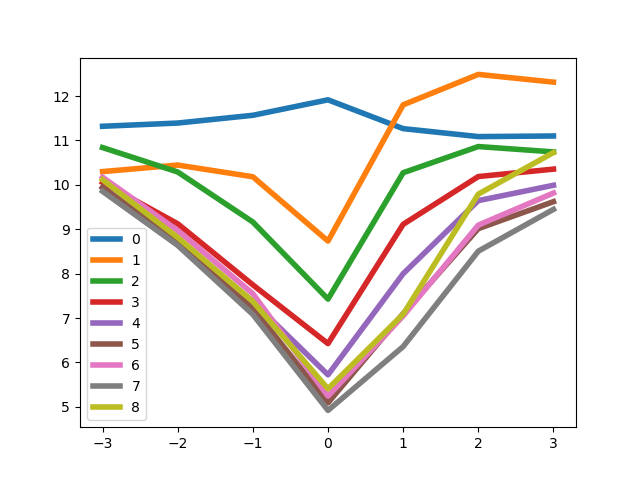
\includegraphics[width=0.48\textwidth]{figures/segmentation-profile-pmis-german-all-heights.png}
\caption{PMIs by syntactic depth.}\label{fig:syntax-depth}
\end{figure}




Qualitative analysis: report proportions of over- and
under-segmentation for our best CNLM, look at common over- and
under-segmentation errors in English (Marco will go manually
through the top 30 most common errors of both types).

\subsection{Discovering morphological categories}
\label{sec:categories}

Focusing on German and Italian given massive morphosyntactic ambiguity
and impoverished morphology of English. Note that these are lexical
properties, probed in a model that has no explicit notion of word!

\paragraph{Word classes (nouns vs.~verbs)}

Procedure as described in the quip.

Baselines: autoencoder, word-based NLM embeddings, also LSTM vs
RNN. Outperforming autoencoder shows that model has learned categories
based on broader distributional evidence, not just typical strings
cueing nouns and verbs.

General accuracy results table for fixed N of training examples as in Table \ref{tab:pos-results}.

\begin{table}[t]
  \begin{center}
    \begin{tabular}{l|l|l}
      \multicolumn{1}{c}{}&\emph{German}&\emph{Italian}\\
      \hline
      LSTM&\ldots&\ldots\\
      RNN&\ldots&\ldots\\
      Autoencoder&\ldots&\ldots\\
      WordNLM&\ldots&\ldots\\
    \end{tabular}
  \end{center}
  \caption{\label{tab:pos-results} \ldots}
\end{table}

Report CNLM vs baseline comparison in function of training examples as in the Quip (possibly for a language only).

\paragraph{Number}

Does the hidden state of the CNLM store an abstract notion of
number. German nouns can be binned in different classes depending on
the morpheme or morphological process they use to form the plural. We
train a number classifier on a subset of these classes, test on the
others: if model generalizes correctly, it means that it knows about
number independently of its surface expression.

Specifics of data-set construction and classifier training. Pick only one setup, e.g., training on -n, -s, and -e.

Baselines/comparisons: LSTM vs RNN, autoencoder, word-based NLM.

Results could be summarized as in Table \ref{tab:number-results}.


\begin{table}[t]
  \begin{center}
    \begin{tabular}{l|l|l|l}
      \multicolumn{1}{c}{}&\emph{training plurals}&\emph{-r}&\emph{no-suffix}\\
      \hline
      LSTM&\ldots&\ldots\\
      RNN&\ldots&\ldots&\ldots\\
      Autoencoder&\ldots&\ldots&\ldots\\
      WordNLM&\ldots&\ldots&\ldots\\
    \end{tabular}
  \end{center}
  \caption{\label{tab:number-results} Figure of merit is accuracy for plural prediction.}
\end{table}


Control follow-up: singular nouns with plural ending (with similar table?).

\subsection{Capturing syntactic dependencies}
\label{sec:dependencies}

Despite not having pre-defined information about words and morphemes,
is the model able to capture non-adjacent syntactic dependencies? NB:
actually for a CNLM even \emph{``\textbf{la} bell\textbf{a}''} is long
distance! Constructions will be language-specific, so we discuss
German and Italian separately (not much in English).

As usual, specifics of training etc that depart from general setup.

\paragraph{German} We consider 4 constructions:
\begin{inparaenum}[i)]
\item article-noun gender agreement, possibly with material in the middle,
\item determiner-noun case concord, again with material in the middle,
\item preposition case sub-categorization, with material in the middle.
\end{inparaenum}


\paragraph{Gender Agreement}
Each German noun belongs to one of three genders (masculine, feminine, neuter), which are morphologically marked on the article.
As the article and the noun can be separated by adjectives and adverbs, we can probe not only the CNLM's knowledge of nouns' genders, but also its ability to model gender agreement across distances.
We create stimuli such as
\begin{tabular}{lllllll}
	\{der, die, das\}& sehr& extrem& rote& Baum \\
	article & adverb & adverb & adjective & noun \\
	the & very & extremely & red & tree
\end{tabular}
where the correct nominative singular article matches the gender of the noun.
We select all nominative singular nouns from the German Universal Dependencies treebank \cite{de2006generating,mcdonald2013universal}, and furthermore all adjectives from the training set.
We construct four conditions varying the number of words between the article and the noun:
We first consider stimuli where no material intervenes.\footnote{Due to syncretism in the article paradigm, there sometimes is ambiguity in the choice of the correct article if the noun's morphology does not uniquely indicate that it is nominative singular. As this affects all feminine nouns, we did not remove such cases. Importantly, this issue is solved as soon as an adjective is present, as their form uniquely indicates that the phrase is nominative singular.}
In the second condition, a randomly selected adjective with the correct (nominative singular) case ending is added.
Crucially, the ending of the adjective does not reveal the gender of the noun.
In the third and fourth condition, one (sehr) or two adverbs (sehr extrem) intervened between the article and the adjective.

In Figure~\ref{fig:gender}, we report accuracy for nouns from each of the three genders and averaged over the genders.
Across genders and conditions, the word-level LSTM tends to perform best, followed by te CNLM.
While the n-gram baseline performs similarly to the CNLM when there is no intervening material, accuracy drops to the random baseline (0.33) in the presence of an adjective.
This can partly be attributed to our choice to choose the adjective randomly from the vocabulary.
Note that this would not be mitigated by models that include interplation with or backoff to lower-order n-grams, as the relevant gender information is present only on the first and last word of each stimulus.
The RNN CNLM is weaker across conditions, and its accuracy drops to random as more intervening material is present.

\begin{figure*}
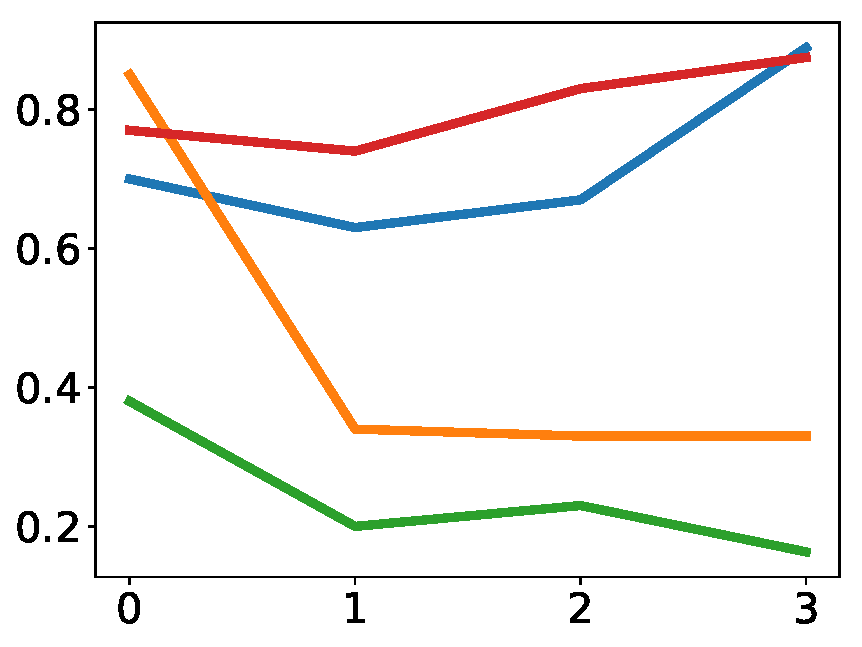
\includegraphics[width=0.24\textwidth]{figures/german-gender-m.pdf}
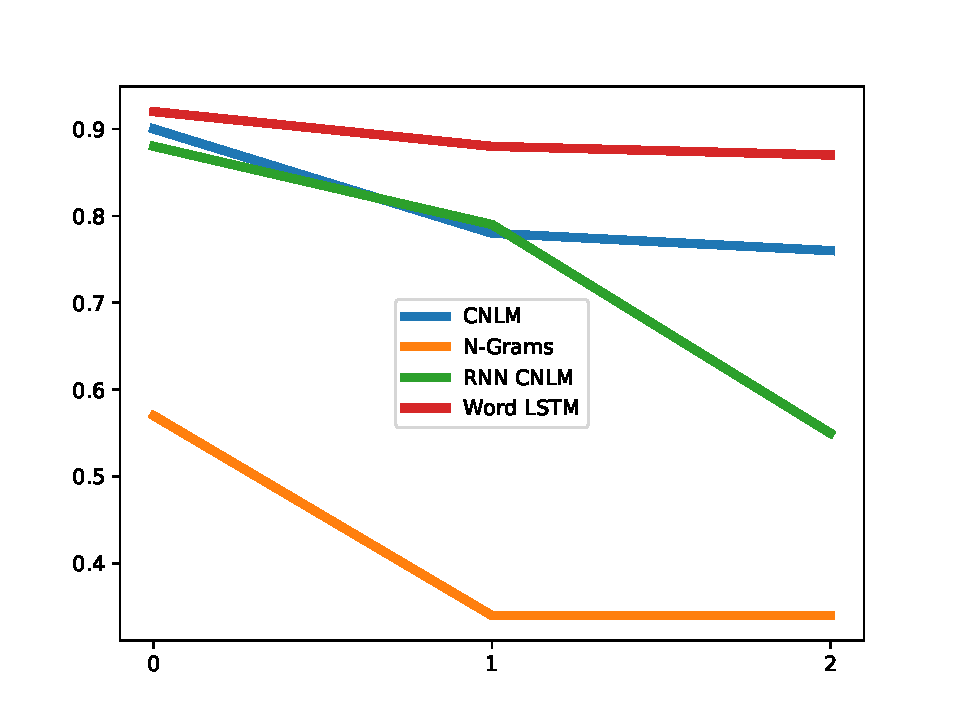
\includegraphics[width=0.24\textwidth]{figures/german-gender-f.pdf}
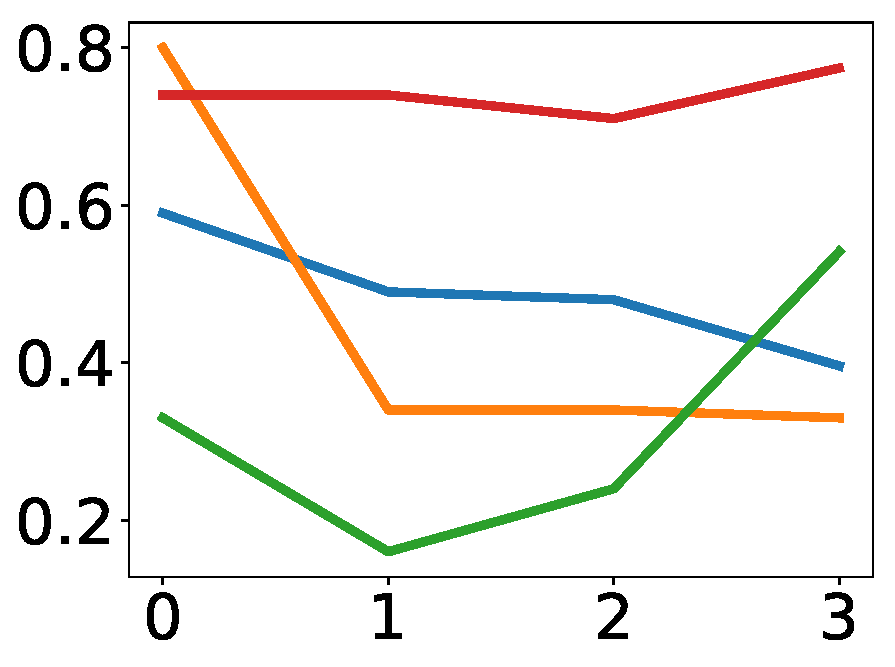
\includegraphics[width=0.24\textwidth]{figures/german-gender-n.pdf}
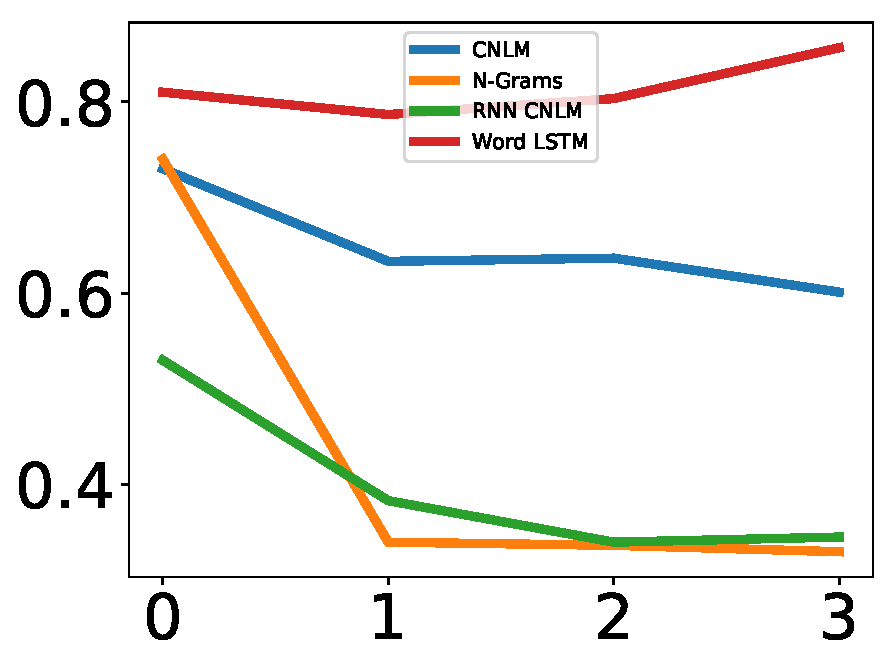
\includegraphics[width=0.24\textwidth]{figures/german-gender-total.pdf}
\caption{Accuracy on the Gender task.}\label{fig:gender}
\end{figure*}


\paragraph{Case Agreement}
Here we test the model's knowledge of case agreement between articles and nouns.
We selected the two determiners dem (dative) and des (genitive), and all nouns  of the appropriate genders that are only compatible with one of the two articles.
Adjectives and adverbs were chosen in the four conditions as in the gender agreement experiment.

Results are shown in Figure~\ref{fig:case}.
Again, the Word LSTM has the strongest overall performance, but the CNLM is competitive as more elements intervene. Accuracy stays well above 80 \% even as three words intervene.
The n-gram model performs well if there is no intervening material, and at chance otherwise.
Accuracy of the RNN CNLM remains above chance for one or two intervening elements, but drops considerably.

Considering the results for the dative and genitive separately, accuracy slightly increases in the dative case and decreases in the genitive case.
This can be attributed to the higher baseline frequency of dative in German, suggesting that both word- and character-based networks are impacted by unigram frequencies as more words intervene.
This effect is far more pronounced for the RNN CNLM, explaining its overall decrease to chance level.
\begin{figure*}
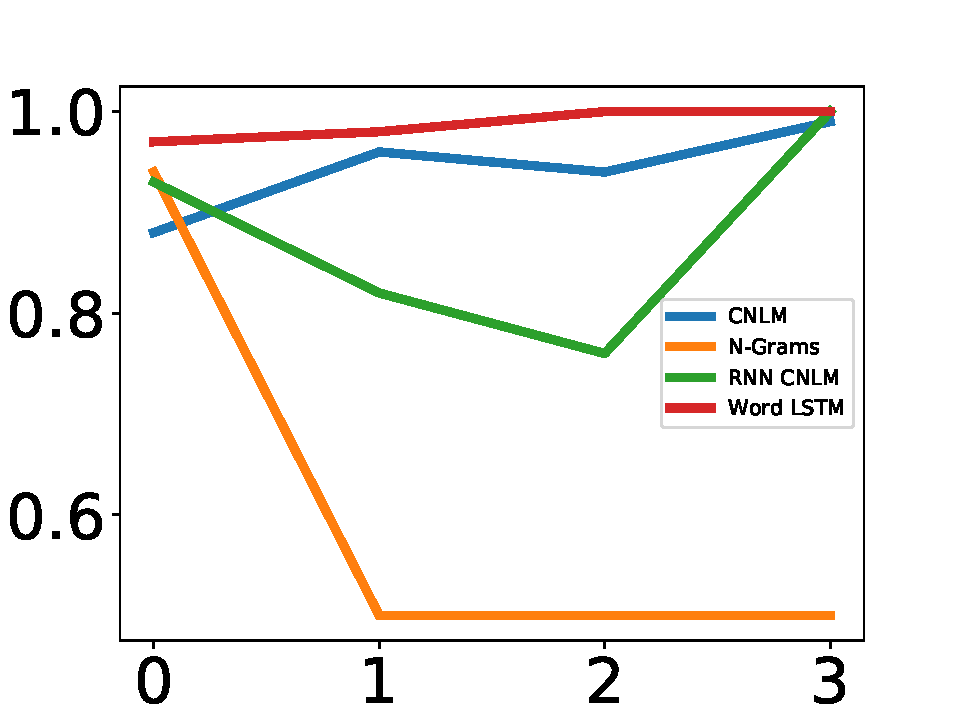
\includegraphics[width=0.24\textwidth]{figures/german-case-Dative.pdf}
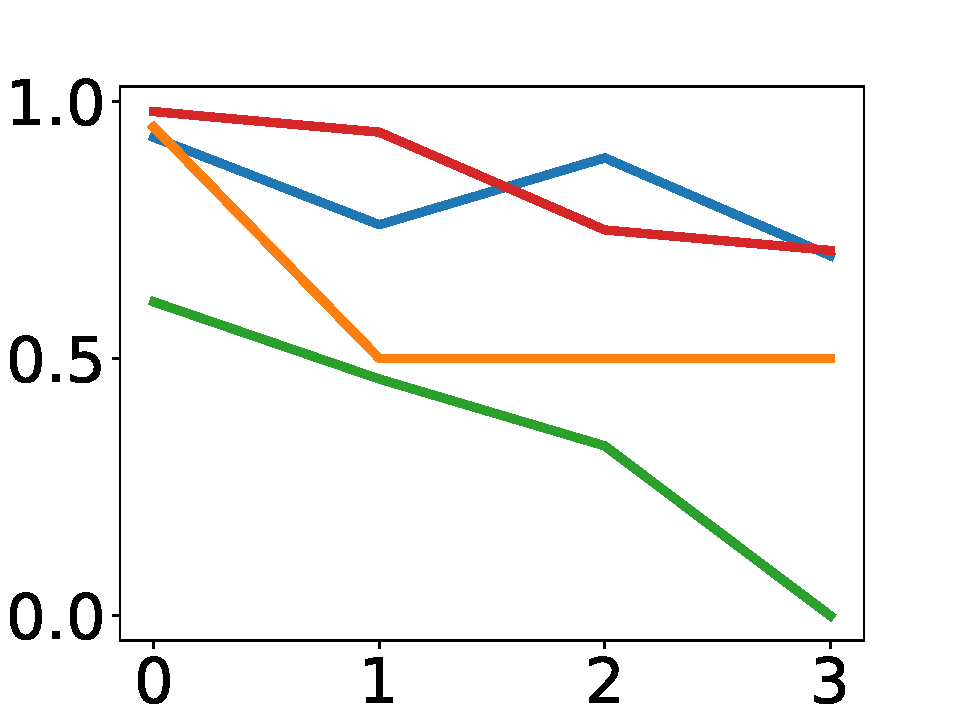
\includegraphics[width=0.24\textwidth]{figures/german-case-Genitive.pdf}
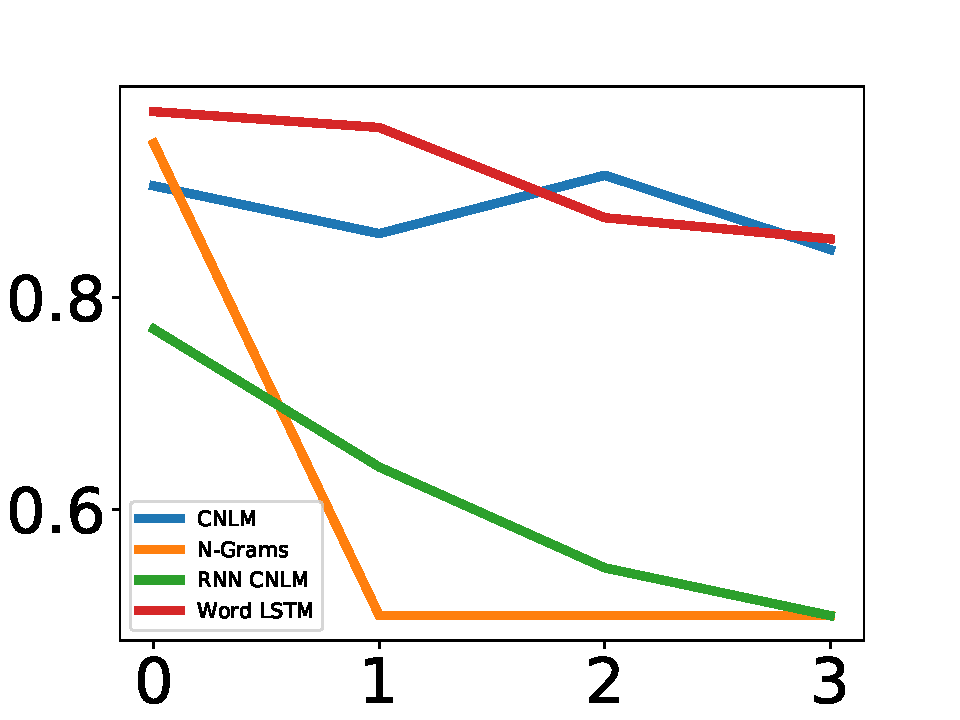
\includegraphics[width=0.24\textwidth]{figures/german-case-total.pdf}
\caption{Accuracy on the Case task.}\label{fig:case}
\end{figure*}

\paragraph{Case Subcategorization}
German verbs and prepositions lexically specify the case appropriate to their objects (mostly dative or accusative).
We probe the CNLM's knowledge of such generalization by considering the preposition \textit{mit} `with', which selects for a dative object.

To focus on knowledge of subcategorization (as opposed to inflectional paradigms), we construct objects whose head noun is a nominalized adjective, whose inflection is very regular.
We take all adjectives that occur at least 100 times in the training data, excluding those that end in -r, as these often reflect lemmatization problems.

We then selected all sentences containing a `mit' prepositional phrase in the German Universal Dependencies treebank, subject to the constraints that (1) the object is not a pronoun, and (2) the object is continuous.
For each sentence, we remove the prepositional phrase and replace it by a phrase of the form
\begin{tabular}{lllllll}
	mit & der & sehr& extrem& \{rote, roten\} \\
	prep & article & adverb & adverb & adjective \\
	with & the & very & extremely & red 
\end{tabular}
where only the -en version of the adjective is compatible with the case requirement of the preposition.
We construct three conditions by varying the presence and number of adverbs, as before.
Note that this correct version is longer than the incorrect one; this ensures that the bias for shorter sequences works against the model.
As a control for baseline probabilities, we also created control stimuli where all words up to the preposition were removed.


We conduct three evaluations: (1) accuracy, (2) accuracy minus accuracy in the control setting, (3) accuracy when classifying based on the log-likelihood ratios between full and control sentences.

\begin{figure*}
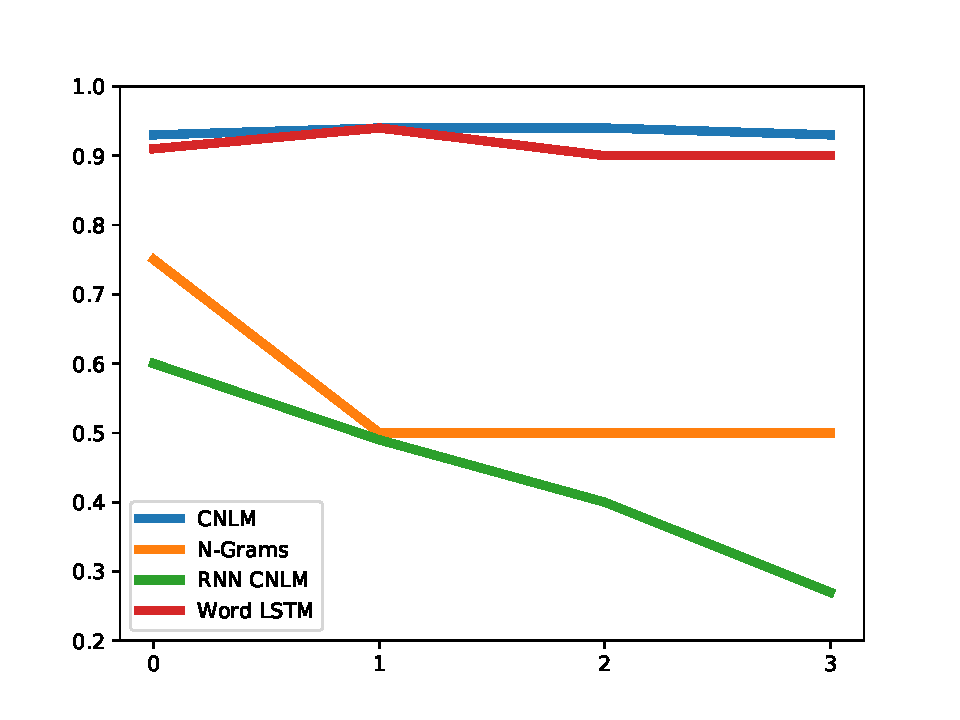
\includegraphics[width=0.24\textwidth]{figures/german-prep-Accuracy.pdf}
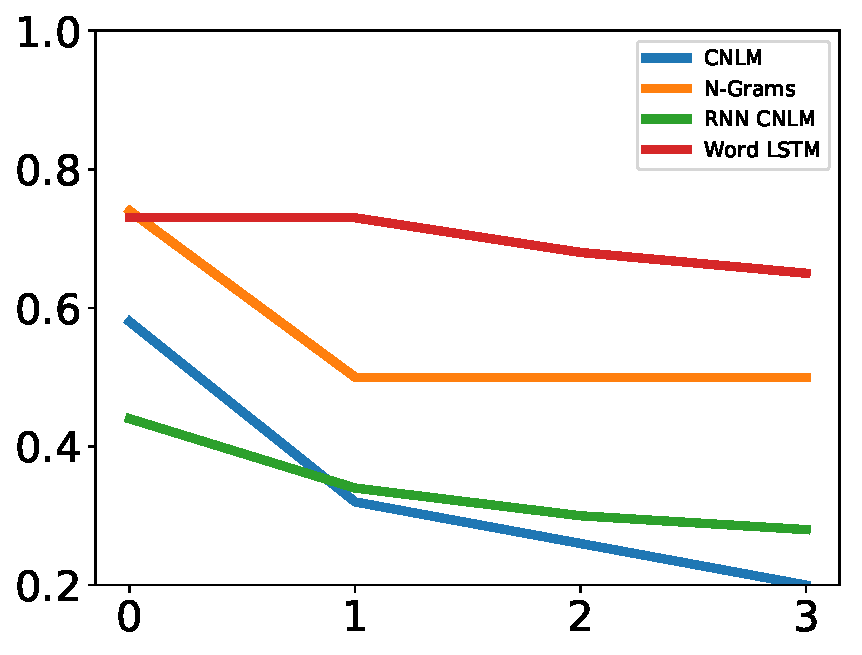
\includegraphics[width=0.24\textwidth]{figures/german-prep-Control.pdf}
\caption{Accuracy on the Case task.}\label{fig:prep}
\end{figure*}

Results are shown in Figure~\ref{fig:prep}.
The CNLM slightly outperforms the word-level language model.
Neither model shows accuracy decay as the number of adverbs increases.
As before, the n-gram model drops to chance as adverbs intervene, while the RNN CNLM starts with low accuracy that decays below chance.


%Discussion case-by-case, including how do we control for possible
%n-gram effects and length. N-gram control: based on counts of each
%stimulus sequence in the corpus.
%
%How to present results: figures, with number of intervening words
%(from 0 to 2 or 3) on x axis, accuracy on y axis. Multiple figures
%when different genders or cases are tested. Within the figures, one
%line per model: LSTM, RNN, n-gram, wordNLM.

\paragraph{Italian} We consider further constructions from Italian,
that confirm the results we got in German. Interesting because we look
at subset of Italian morphology where gender and number are explicitly
encoded while allowing for tightly controlled comparison of
same-length strings, limited to stimuli unseen in training corpus.
\begin{inparaenum}[i)]
\item article-noun gender agreement with material in the middle,
\item article-adjective gender agreement, with an adverb in the middle,
\item article-adjective number agreement, with an adverb in the middle.
\end{inparaenum}

\paragraph{Article-Noun Gender Agreement}
(1) eadj-aonoun: adjective ending in -e + noun that has both a masculine (-o) and feminine (-a) version.

we created \{il, la\} ADJ NOUNo, and \{il, la\} ADJ NOUNa

None of the pairs appear in the training data, and all single words appear at least 100 times.
Further, the nouns in -a and  -o have reasonably balanced frequency (neither form is twice more frequent than the other), or they are both frequent (appear at least 500 times)
Also, we considered only -e adjectives that occur at least with 10 different nouns in the prenominal position, as this is somewhat marked in Italian/


\paragraph{Article-Adjective Gender Agreement}
(2) adv-aoadj: il ADVERB \{ADJo, ADJa\}, la ...

only adjectives that occurred 1K times in the training corpus, as this is the most common kind of adjective in Italian.
We excluded all cases in which the adverb-adjective combination occurred in the training corpus, in either feminine or masculine form.

\paragraph{Article-Adjective Number Agreement}
(3) adv-aeadj: la ADV \{ADJa, ADJe\}, le ADV \{ADJe, ADJa\}

Similar here, but we took a 500-occurrences threshold, as feminine plurals are less common.
Further, we manually removed adjectives that did not combine well semantically with the adverbs under consideration (pi{\`u}, meno, tanto).


Results are shown in Table~\ref{tab:ital-agr-results}.
The word LSTM shows the highest overall performance, closely followed by the LSTM CNLM.
The RNN performs well on adjective gender, and considerably worse than the CNLM on the other tasks.
For the CNLMs, the most challenging task was article-noun gender agreement.



\begin{table}[t]
  \begin{center}
    \begin{tabular}{l|l|l|l|l}
      \multicolumn{1}{c}{}&\emph{LSTM CNLM}&\emph{RNN CNLM}&\emph{Word LSTM}\\
% eadj-aonoun
	    Noun Gender & 97/90  & 84/73 & 99/96 \\
%      adv-aoadj
	    Adj. Gender & 99/100 & 100/97 & 98/100 \\
% adv-aeadj
	    Adj. Number & 99/99 & 99/70 & 100/100 \\
    \end{tabular}
  \end{center}
  \caption{\label{tab:ital-agr-results} Results for morphosyntactic tests in Italian}
\end{table}





%Discussion case-by-case, including how we control for n-gram frequency
%and length.
%
%Results table with a row for each pattern and a column for each model.


\subsection{Lexical semantic similarity}
\label{sec:similarity}

In English, because that's where we have resources available.

Correlation with one or more word similarity sets.

Comparison to word-based NLM (rather than word2vec or such, which is
specifically tuned for semantics).

